
\subsubsection{Contact Angle Goniometer (Verison 1)}
Preliminary designs of my contact angle goniometer implement a radiative temperature control box which encloses an argon gas filled container where the sample resides, as seen in Figure \ref{fig:rad-temp-box}.  The presence of argon is meant to prevent any further oxidation of the Galfenol sample as well as the gallium droplet. The container was initially made of a clear acrylic plastic, but prolonged exposure to temperatures above 80\degree C caused thermal deformation of the plastic making longer experiments impossible to perform without environment contamination.  A clear pyrex container replaced the acrylic box to fix this issue.  Application of the liquid gallium drop to our surfaces was done via a mounted plastic syringe with disposable stainless steel hypodermic needles that were available at the time. Liquid gallium tends to adhere strongly to the stainless steel needle tips which makes wetting to the sample very difficult. The stainless steel tip tends to deform the highly viscous gallium drop resulting in non-uniform hemispheric drop shapes, as shown in Figure \ref{fig:deformed-ga}.
\begin{figure}[h]
	\centering
	\begin{subfigure}[c]{0.45\textwidth}
		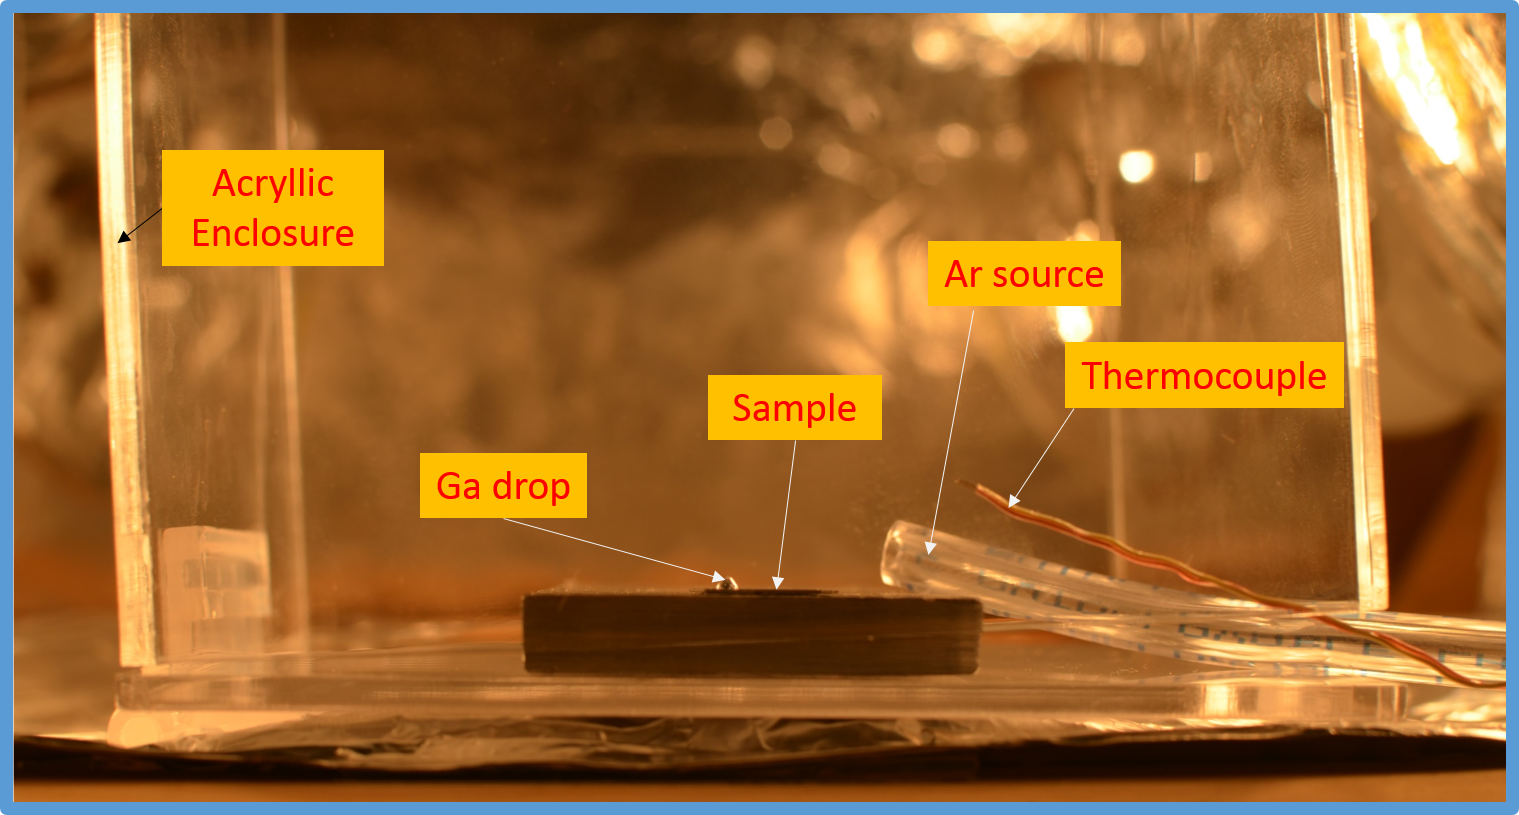
\includegraphics[width=\linewidth]{rad-temp-box}
		\subcaption{~}
		\label{fig:rad-temp-box}		
	\end{subfigure}
	\begin{subfigure}[c]{0.45\textwidth} 
		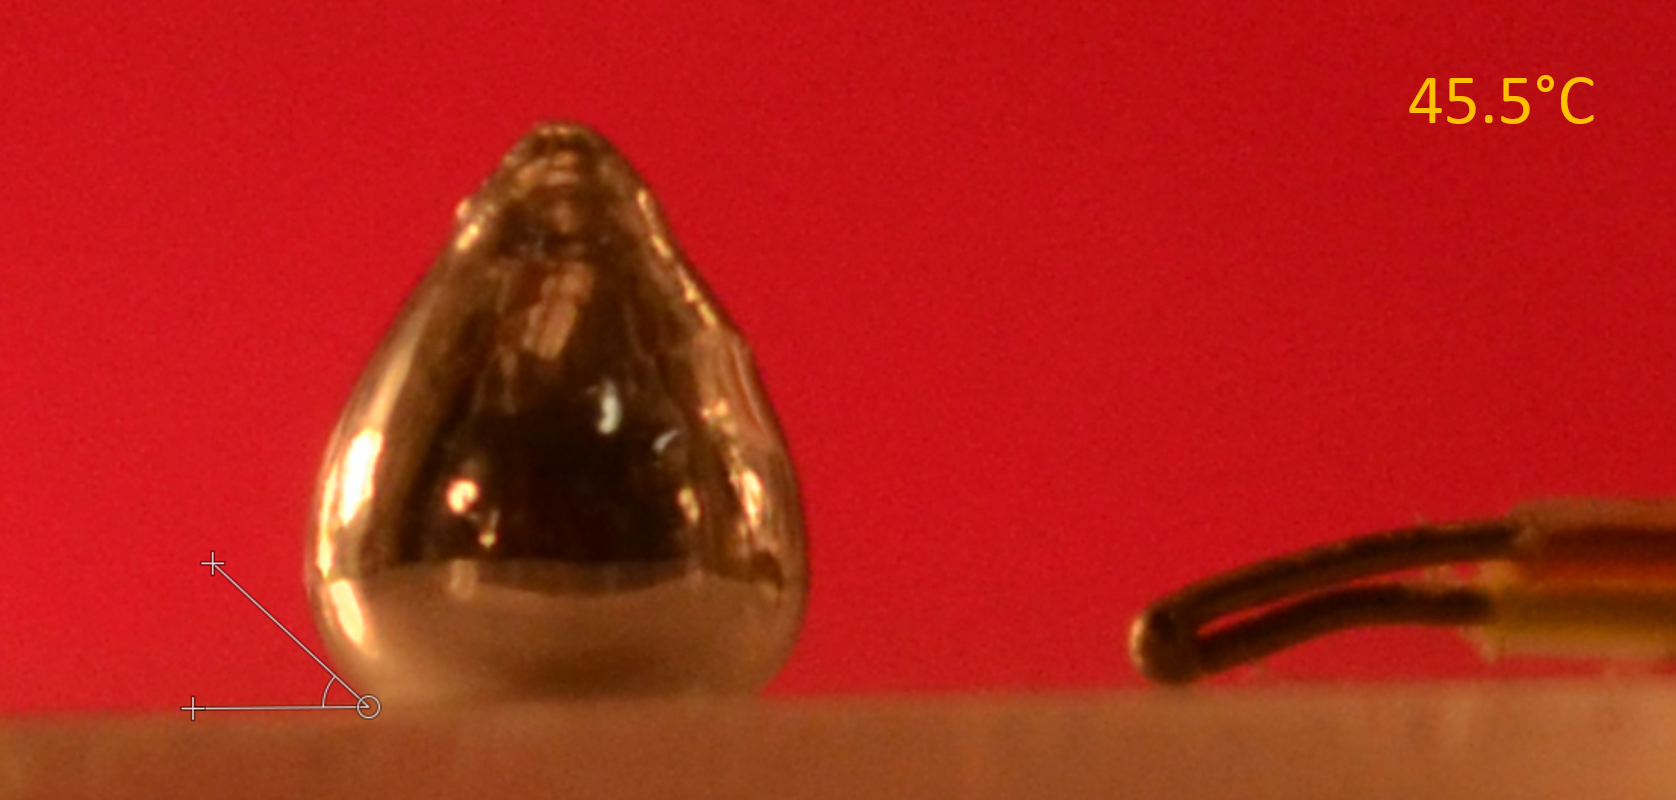
\includegraphics[width=\linewidth]{deformed-ga}
		\subcaption{~}
		\label{fig:deformed-ga}		
	\end{subfigure}
	\caption{(a) The first design of our contact angle goniometer.  The acrylic container houses the argon environment and sample.  This design was modified with a more stable glass enclosure. (b) A highly deformed gallium drop next to the thermocouple on a ceramic YAG test sample at 45.5\degree C.}
	\label{fig:prelim-design}
\end{figure}

For this experiment to succeed, a number of challenges were overcome. The simplest task involved polishing Galfenol samples using incrementally higher grit SiC paper and subsequent 0.1 $\mu$m colloidal silica particles to decrease the roughness to below 40 nm, as proven using AFM measurements. %TODO: Find AFM roughness picture?
% AFM roughness pic
%\begin{figure}
%	\centering
%		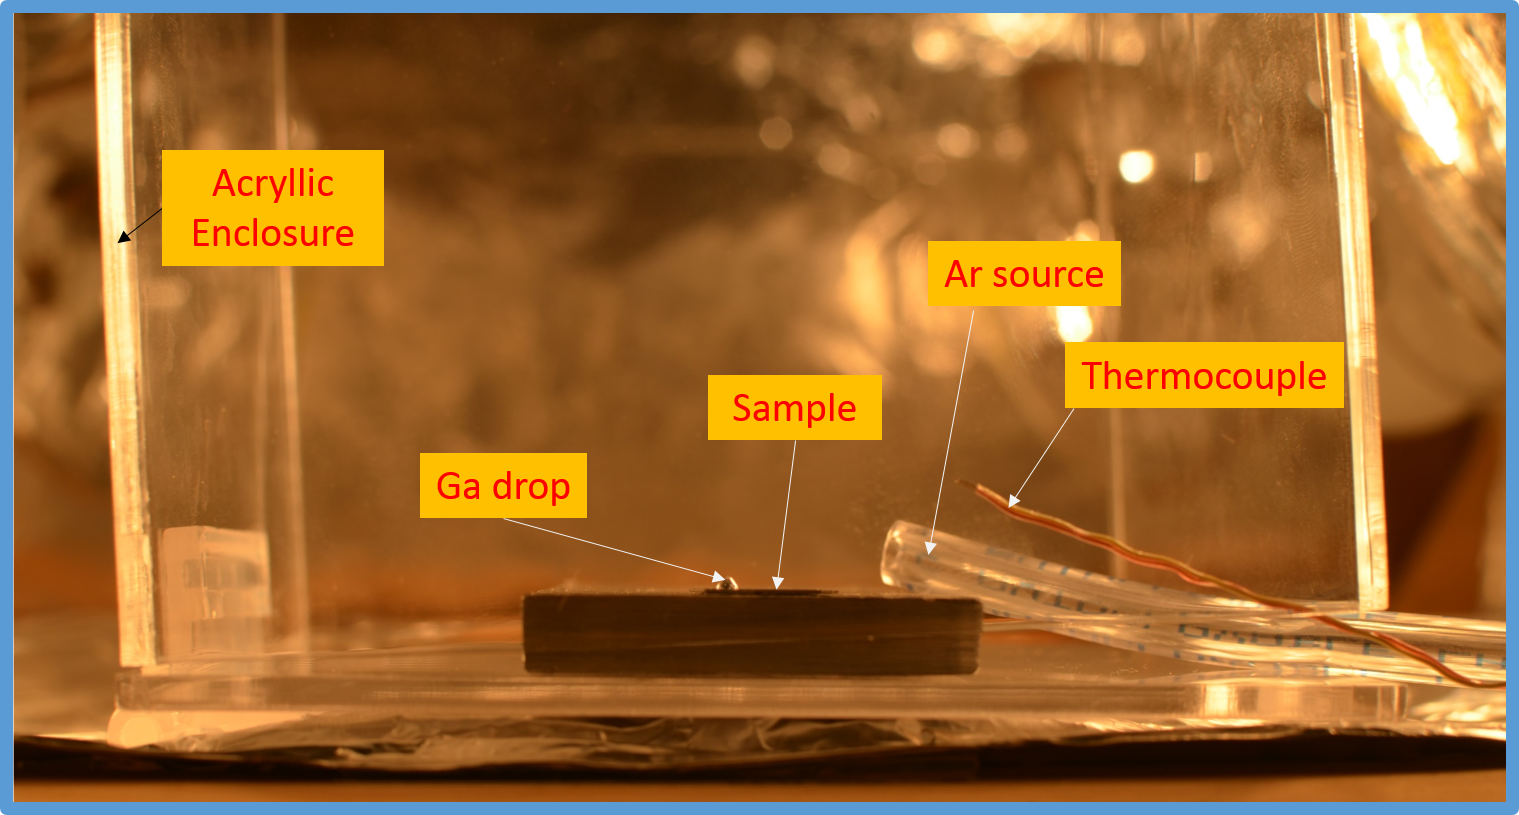
\includegraphics[width=\linewidth]{rad-temp-box}
%	\caption{(a) The first design of our contact angle goniometer.  The acrylic container houses the argon environment and sample.  This design was modified with a more stable glass enclosure. (b) A highly deformed gallium drop next to the thermocouple on a ceramic YAG test sample at 45.5\degree C.}
%	\label{fig:prelim-design}
%\end{figure}
The radiative box that housed this experiment had a high variability in temperature according to thermocouple readings, so a smaller apparatus with a top-side syringe opening is made to properly perform gallium drop tests at specific temperatures and prevent interaction with the experiment environment. There must also be bright white backlighting to obtain a high contrast drop profile. In this radiative box configuration, the high-reflecting liquid metal surface prevents a high contrast drop profile image, as seen in Figure \ref{fig:deformed-ga}. Proper contact angle measurements also require the gallium droplets to carefully wet the surface while forming an axisymmetric and spherical-like shape on the solid surface. A height adjustment system must be used to move the gallium pendant drop close enough to the sample surface for solid adhesive forces to overcome the adhesion to the needle. Lastly, the argon gas environment could be more well contained, instead of just filling up the glass sample enclosure from the bottom and spilling out the top due to higher density argon displacing the surrounding air environment. 

\subsubsection{Version 2}
\begin{figure}
	\centering
	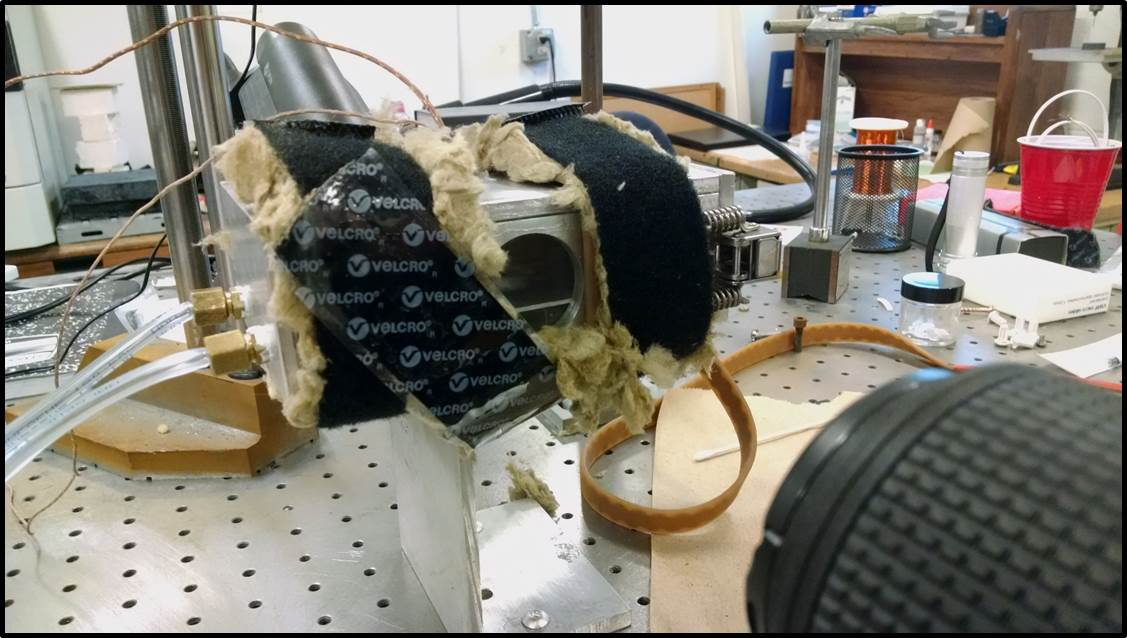
\includegraphics[width=\linewidth,trim={0 0 0 1cm}]{enviro_chamber}
	\caption{The second version of our gallium contact angle goniometer. The aluminum enclosure conductively transfers heat, the gas lines flow Ar gas into the chamber, top-mounted thermocouples monitor the gas and sample temperature, and the glass windows allow for backlighting of the drop profile along with high resolution image capture using a DSLR camera.}
	\label{fig:enviro_chamber}
\end{figure}
The new experimental apparatus can be seen in Figure \ref{fig:enviro_chamber}. The main structure is made of aluminum with two round glass windows on the front and back. The aluminum is meant to conductively transfer heat to the substrate by means of a heating cable wrapped around the outside of the structure. The high thermal conductivity of aluminum allows for a quick transfer of heat, thus an increased control of sample temperature. The time percentage dial controller attached to the heating tape is calibrated with the sample temperature using a thermocouple placed on the sample surface. Sample temperature can be consistently controlled with $\pm$0.5\degree C accuracy. Backlighting greatly improved the drop profile contrast by having only one white light source coming from one side of the droplet, as seen in Figure \ref{fig:deformed_ga}. The Ar environment is also far more contained and controlled. The silicone sealant creates a nearly air-tight system where the argon will displace all gas contaminants that could oxidize the sample or gallium droplet. 
%These precautions are suitable for any metals samples tested because each sample is polished according to the procedure described above and then cleaned with acetone to remove any oxides. 
Once the sample is inserted and sealed in the environmental chamber, the Ar prevents oxidation throughout the experiment. 
%A positive partial pressure is achieved in the chamber with an in- and out-valve. %TODO find more sufficient answer to how this removes oxides. 

While extensive steps have been taken to inhibit oxidation on the metal surfaces, preventing oxidation on the surface of liquid gallium was a greater challenge. Pure gallium and Gallium-based alloy surfaces instantly oxidize in ambient environments, turning into a thin layer of gallium oxide (Ga$_{2}$O$_{3}$ and Ga$_{2}$O).\cite{Regan1995,Regan1997,Scharmann2004} This oxide layer is solid and remains elastic until it experiences a yield stress. Therefore, that an oxidized gallium droplet does not behave as a simple liquid, but as a viscoelastic material. In addition, the oxide layer of gallium is known to adhere to almost any solid surface, causing a severe stiction problem that interferes with interfacial energy measurements.\cite{Scharmann2004}. This shows how dramatically the gallium surface tension decreases when the oxide forms. Khan \etal showed that gallium oxide forms hydroxyl groups on their exterior surface, making the drops lyophilic as opposed to the expected lyophobic behavior of pure gallium, a high surface tension liquid.\cite{Hardy1985,Alchagirov2005} 

\begin{figure}
	\centering
	\begin{subfigure}[c]{0.45\textwidth}
		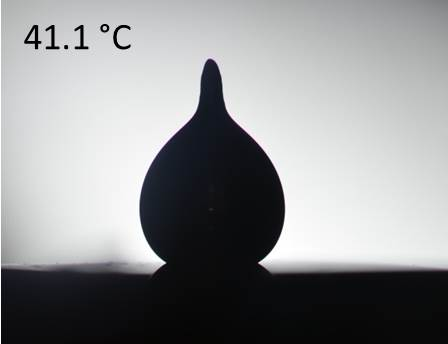
\includegraphics[width=\linewidth,trim={0 0 0 0}]{ga_41c}
		\subcaption{~}
		\label{fig:ga_41c}		
	\end{subfigure}
	\begin{subfigure}[c]{0.45\textwidth} 
		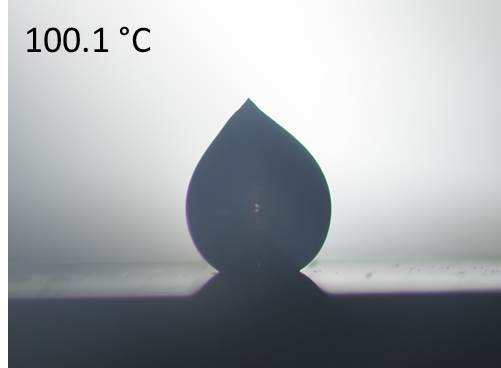
\includegraphics[width=\linewidth,trim={0 0 0 0}]{ga_100c}
		\subcaption{~}
		\label{fig:ga_100c}		
	\end{subfigure}
	\caption{Pure liquid gallium obtains viscoelastic properties when trace amounts of oxygen are present via formation of oxide shell. Non-axisymmetric Ga drops form on this iron substrate.}
	\label{fig:deformed_ga}
\end{figure}
Figure \ref{fig:deformed_ga} shows our direct observation of this phenomenon with teardrop shaped droplets formed by adhering to the iron surface while still being pulled upwards by the deposition needles. The general shape of these drops were unchanged for many hours even at temperatures approaching $\sim$100\degree C, thus exhibiting the stability of viscoelastic properties caused by the solid oxide layer. Removing the oxide layer from liquid gallium will return normal liquid properties to gallium and allow the use of axisymmetric drop analysis calculations: Young-Laplace equation, 
%todo: [NEED MORE TECHNIQUES FROM KRUSS GONIOMETER]



Oxide removal permits liquid gallium to directly interact with metal surfaces instead of gallium oxide; the derived terms for \gamSL and \gamLV in Equation \ref{youngs-eqn-ga} become more robust. A number of techniques have been developed to remove and recover gallium oxide on liquid gallium: ultra-high vacuum (UHV) techniques,\cite{Regan1995,Regan1997} chemical vapor etching,\cite{Kim2013,Doudrick2014} and electrohydrodynamic phenomena.\cite{Khan2014} A chemical vapor etch is the best option for this experiment because it has a minimal effect on the surface of metals and the experimental apparatus does not need to be changed. To execute the vapor etch, a pendant drop of gallium was formed and a pipette of 37wt\% HCl was brought in close proximity to etch away the oxide layer. The same procedure was performed on the sessile drop of gallium on the desired surface to etch away any oxide left on top of the droplet, as seen in Figure \ref{fig:hcl_vapor_treat}. The contact angles of gallium on bare glass before and after HCl vapor treatment are similar to respective contact angle values in Kim \etal\cite{Kim2013}

\begin{figure}
	\centering
	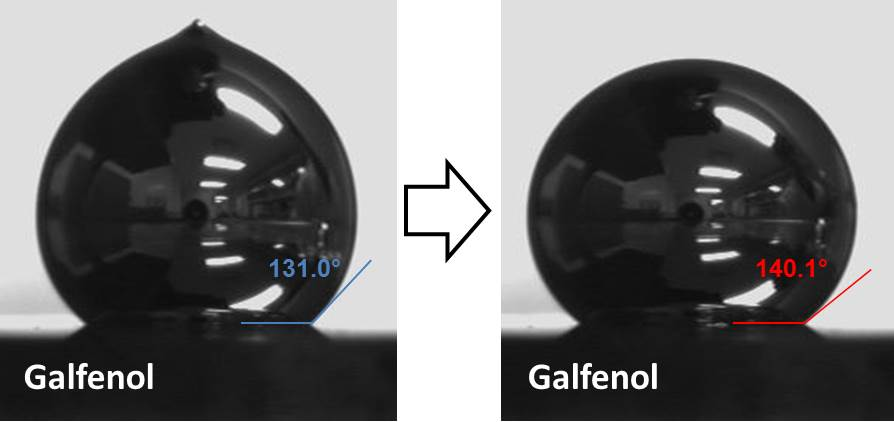
\includegraphics[width=\linewidth,trim={0 0 0 1cm}]{hcl_vapor_treat}
	\caption{This image shows the contact angle of gallium on a Galfenol sample in an argon environment before and after HCl vapor treatment.}
	\label{fig:hcl_vapor_treat}
\end{figure}

With the HCl vapor treatment added to the procedure, temperature-varying gallium contact angle measurements in an argon environment were executed in the aluminum chamber on multiple metal substrates. Polycrystalline samples of high purity ($>$99.99\%) tin, copper, and iron were polished and had liquid gallium deposited on their surfaces. The temperature in the chamber was slowly ($<$10\degree C/min) increased from ~30\degree C to just below 100\degree C. Beyond 100\degree C, the heating tape becomes inconsistent with the intervals of heat applied to the chamber. Photographs of gallium drop profiles are taken at ~10\degree C intervals to observe progression of the drop shape as temperature increases. The same procedure is done as the temperature is decreased to 30\degree C to observe reversibility of this process, since we assume that the thermal expansion of the substrate drives the change in \gamSL from Equation \ref{youngs-eqn-ga}. 

It is known that liquid gallium tends to corrode most metal surfaces.\cite{Lewandowski2015,Narh1998,Fitzgerald1999} Since experiments lasted for less than one hour, corrosion between the two metals should not be significant enough to effect the measurement. For the polycrystalline tin and copper samples, gallium began to visibly corrode through the surface between 60\degree C and 70\degree C, as evident by a rapid contact angle decrease on only side of the drop profile. Polycrystalline iron samples did not experience corrosion problems throughout the experiments. It is expected that as the temperature increases, the thermal expansion of the solid will isotropically expand the drop thus decreasing the contact angle. Some gallium contact angles decrease on iron, but it is often that the decrease occurs on one side of the drop profile as the temperature increases. This is most likely due to the polycrystalline grains having different thermal expansions, hence the drop spreading is anisotropic. This suggests that a single-crystal grain or highly-textured surface grain is needed to properly observe an isotropic drop expansion. 


Since the iron sample did not corrode in the presence of gallium, we proceeded to a Galfenol sample with an abnormally grown \hkl(110) grain. Figure \ref{fig:ca_ebsd} shows the location of a gallium droplet in contact with the highly Goss-textured surface. Using the same temperature intervals, the right and left contact angles were measured and the surface energy
\begin{figure}
	\centering
	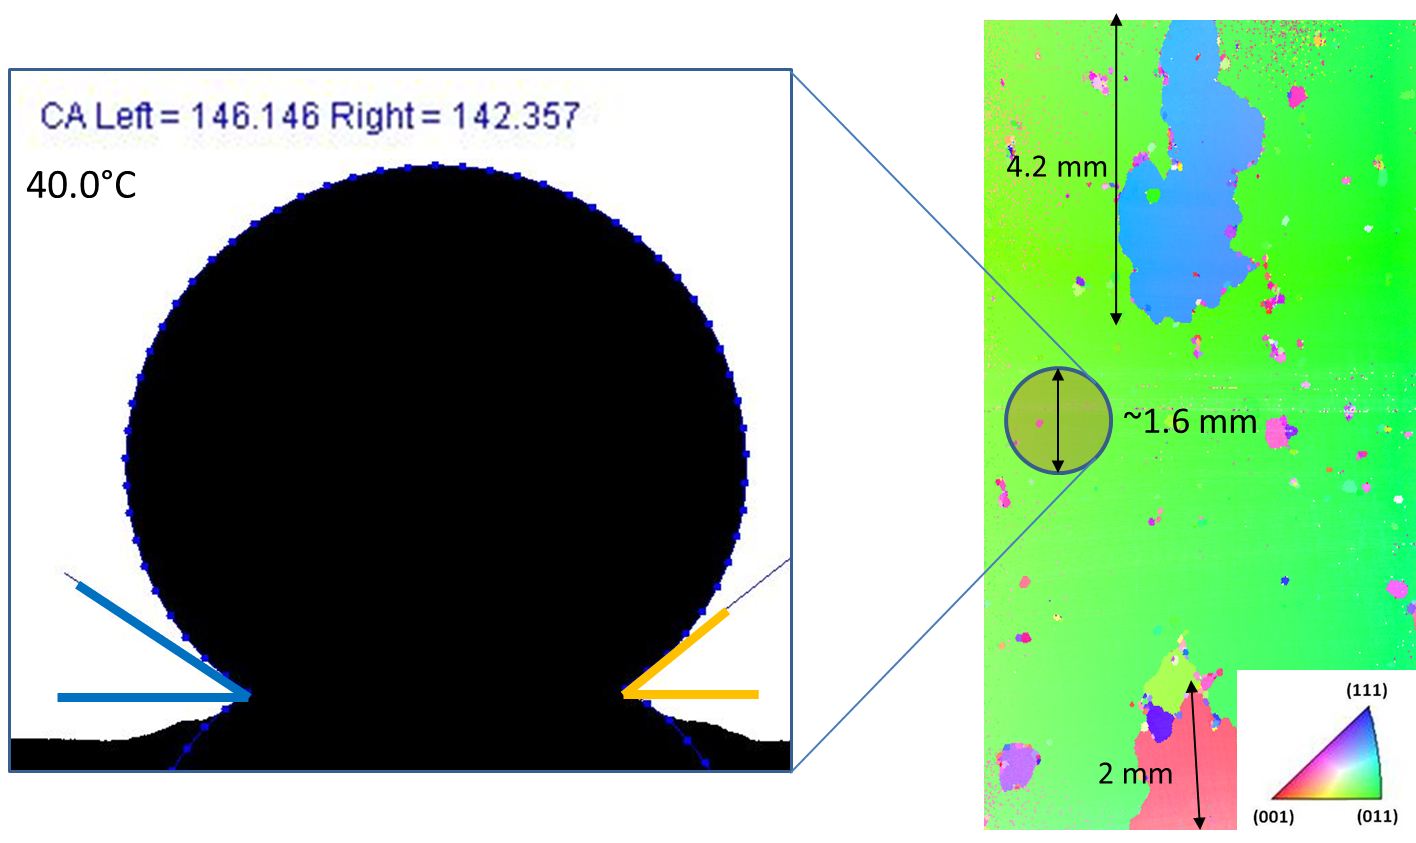
\includegraphics[width=\linewidth,trim={0 0 0 2cm}]{ca_ebsd}
	\caption{The location of a gallium drop on highly Goss-textured surface.}
	\label{fig:ca_ebsd}
\end{figure}
 was calculated using Equation \ref{youngs-eqn-ga}. The contact angle measurements and surface energy calculations are shown in Figure \ref{fig:goss_se_msrmnt}. The contact angle measurements show anisotropic spreading behavior since the left contact angle recedes as temperature increases while the right contact angle advances. At 60.7\degree C, the contact angles reached close to the same value which may indicate an equilibrium point of combating thermal expansions caused by nearby island grains. 

 The increasing surface energy trend as the temperature increased was not an expected result. As the temperature of a metal surface increases, the cohesive force binding atoms will decrease because the atoms will vibrate more rapidly. Since surface energy depends on the net inward cohesive force, a decrease in surface energy with increasing temperature was expected. Moreover, such a high difference in surface energy as the temperature increased was not expected. The $ \gamma_{SL}(T) $ term is extremely dominant compared to the $ \gamma_{LV}(T) $ term. This is due to the high Young's modulus value associated with Galfenol. The values of surface energy for the \hkl(110) Galfenol grain are two orders of magnitude greater than predicted values of $\alpha$-iron, \gamSV = 2.0535 J/m$^2$.\cite{Wang2000} 
\begin{figure}[h]
	\centering
	\begin{subfigure}[c]{0.47\textwidth}
		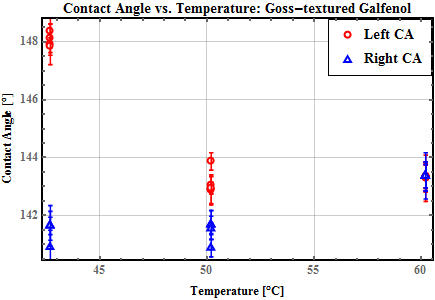
\includegraphics[width=\linewidth]{CAvsTemp_Goss-Galfenol3}
		\subcaption{~}
		\label{fig:goss_ga_ca}		
	\end{subfigure}
	\begin{subfigure}[c]{0.47\textwidth} 
		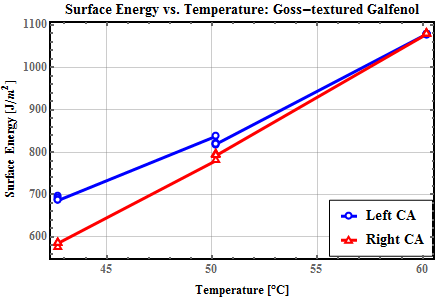
\includegraphics[width=\linewidth]{SEvsTemp_Goss-Galfenol3}
		\subcaption{~}
		\label{fig:goss_ga_se}		
	\end{subfigure}
	\caption{(a) Blue and red dots show left and right contact angle, respectively, of liquid gallium on \hkl(110) Fe-Ga. (b) Calculated surface energy values of \hkl(110) Fe-Ga grains using Equation \ref{youngs-eqn-ga}.}
	\label{fig:goss_se_msrmnt}
\end{figure}
 After presenting these preliminary findings at the XXIV International Materials Research Congress and 2015 MRS Fall Meeting,\cite{VanOrder2015a,VanOrder2015} I discussed possible avenues of improvement for the gallium contact angle experiment with colleagues and potential collaborators. A more concrete measurement of \gamSL between liquid gallium and solid would need to be examined, a very non-trivial task. Ultimately, we decided to suspend the gallium drop experiment and re-evaluate the measurement strategy. 
 %for obtaining orientation-dependent surface energies of magnetostrictive materials. 
 
Overall, this was an exploration of well-proposed and innovative research. Assumptions were made about how the system would interact and efforts to achieve good results in the lab were made. It was determined that these assumptions were too great and the experiment failed to meet expectations. Much was learned about the complexity of surface energy research from both a theoretical and experimental perspective. This failure persuaded me to find a more robust and promising method for accomplishing project goals within the constraints of orientation-dependent surface energy characterization. 
%TODO: don't say failure in the last sentence. Find a different way to build yourself up.


